\documentclass{article}
\usepackage[utf8]{inputenc}
\usepackage{moreverb}

\usepackage[T1]{fontenc}
\usepackage{lmodern}
\usepackage{microtype}
\usepackage[french]{babel}
\usepackage{listings}
\usepackage{graphicx}
\usepackage{subcaption}
\usepackage{placeins}

\usepackage[toc]{glossaries}

\usepackage[hidelinks]{hyperref}

\usepackage{color}   

\lstset{
	tabsize=2,
	breaklines=true,
	numbers=left,
	float=[!htb],
	basicstyle=\small,
	numberstyle=\tiny,
	language=C,
	morekeywords={acc},
	aboveskip=5mm,
	belowskip=5mm,
	framexleftmargin=16pt,
	framextopmargin=6pt,
	framexbottommargin=3pt,
	frame=tblr,
	captionpos=b,
}

\title{Portage de codes C sur \textit{GPU} avec OpenACC}
\author{Quentin KREMPP}

\makeglossaries

\newglossaryentry{flops}
{
	name=FLOPS,
	description={Le nombre d'opérations en virgule flottante par seconde (en anglais : floating-point operations per second ou \textit{FLOPS}) est une unité de mesure de la performance d'un système informatique. Les opérations en virgule flottante (additions ou multiplications) incluent toutes les opérations qui impliquent des nombres réels.\cite{Wiki:flops}}
}

\newglossaryentry{cpu}
{
	name=CPU,
	description={Un processeur (ou unité centrale de traitement, \textit{UCT} ou en anglais central processing unit, \textit{CPU}) est un composant présent dans de nombreux dispositifs électroniques qui exécute les instructions machine des programmes informatiques.\cite{Wiki:cpu}}
}

\newglossaryentry{gpu}
{
	name=GPU,
	description={Un processeur graphique, ou \textit{GPU} (de l'anglais Graphics Processing Unit), est un circuit intégré présent la plupart du temps sur une carte graphique et assurant les fonctions de calcul de l'affichage. Un processeur graphique a généralement une structure hautement parallèle qui le rend efficace pour une large palette de tâches graphiques.\cite{Wiki:gpu}}
}

\newglossaryentry{cuda}
{
	name=CUDA,
	description={(initialement l'acronyme de Compute Unified Device Architecture) est une technologie de GPGPU (General-Purpose Computing on Graphics Processing Units), c'est-à-dire utilisant un processeur graphique pour exécuter des calculs généraux à la place du processeur. Ce langage de programmation permet de programmer des \textit{\gls{gpu}} en \textit{C}.\cite{Wiki:cuda}}
}

\newglossaryentry{pci}
{
	name=PCI,
	description={L'interface \textit{PCI} (de l'anglais Peripheral Component Interconnect) est un standard de bus local (interne) permettant de connecter des cartes d'extension sur la carte mère d'un ordinateur.\cite{Wiki:pci}}
}

\newglossaryentry{coeur}
{
	name={cœur},
	description={Un cœur physique est un ensemble de circuits capables d’exécuter des programmes de façon autonome. Toutes les fonctionnalités nécessaires à l’exécution d'un programme sont présentes dans ces cœurs.\cite{Wiki:coeur}}
}

\newglossaryentry{paral}
{
	name=parallélisation,
	description={Le parallélisme consiste à mettre en œuvre des architectures d'électronique numérique permettant de traiter des informations de manière simultanée, ainsi que les algorithmes spécialisés pour celles-ci.\cite{Wiki:paral}}
}


\begin{document}

\begin{figure}[!htb]
	\minipage{0.32\textwidth}
  
\includegraphics[height = 120pt]{Ensta.jpg}
	\endminipage\hspace*{4cm}
	\minipage{0.32\textwidth}
  
\includegraphics[height = 50pt]{Inria.png}
	\endminipage
\end{figure}



    %\bigbreak    
    %\bigskip
    
        
    \begin{center}
        \Large
        \textbf{Projet de recherche (PRe)}\\
        \large
        \textbf{Majeure : Mathématiques appliquées}\\
        \textbf{Année scolaire : 2020}\\
        
    \bigbreak 
        
        \huge
        \textbf{Plus de science pour moins de code : Portage de codes C sur GPU avec OpenACC}\\
        
        
    \end{center}
        
    %\bigbreak
    %\bigskip
    %\bigbreak
    \begin{center}
        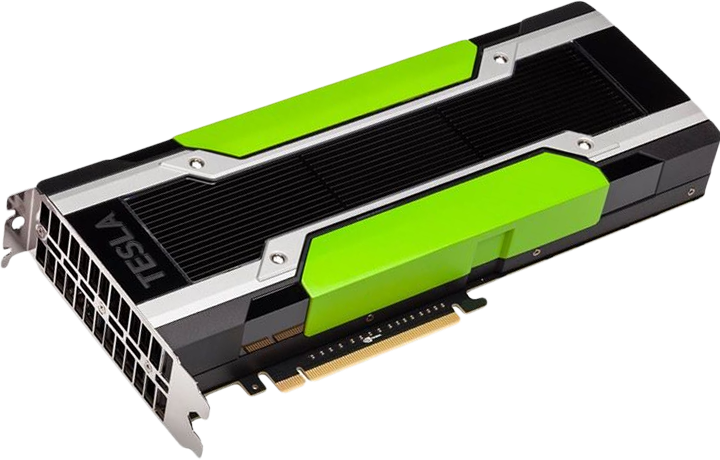
\includegraphics[height = 150pt]{GPU.png}
    \end{center}
    
    \begin{center}
        \color{red}{
        \framebox[2\width]{\huge{Non-confidentiel}}
        }
    \end{center}
    
 
    
    \large
    
        \textbf{Auteur : KREMPP Quentin} \hfill \textbf{Promotion : 2021}
    
    %\bigbreak
    %\bigskip
    
    \begin{center}
    
        \textbf{Tuteur ENSTA Paris : ALES Zacharie}\\
        \textbf{Tuteur dans l'organisme d'accueil  : MODAVE Axel}
    
    %\bigbreak
    \bigskip
    %\bigbreak
    
    \normalsize
        \textbf{Stage effectué du 18/05/2020 au 31/07/2020}\\
    
        \textbf{Organisation d'accueil : Equipe POEMS - Ensta Paris, Inria, CNRS}\\
        \textbf{Adresse : 828 Boulevard des Maréchaux, 91120 Palaiseau}
     
    \end{center}

\newpage

\frontmatter

\tableofcontents

\newpage

\section{Note de non confidentialité}

Ce document est non confidentiel. Il peut donc être consulté en ligne par tous.

\newpage

\section{Remerciements}

Je remercie chaleureusement Axel MODAVE de m'avoir proposé ce sujet qui s'est avéré très enrichissant, et pour le suivi qu'ils m'ont offert avec Luis MALTEZ FARIA malgré les circonstances inhabituelles de cette crise sanitaire. Ils m'ont accompagné tout au long de ce projet, m'ont orienté et m'ont permis de produire un travail dont je suis fier. Je remercie aussi ceux qui m'ont entouré pendant la durée de mon télétravail quand il n'était pas tout les jours facile de se mettre au travail, Claire, Antoine et Théo.

\newpage

\section{Résumé}

L'objectif de ce travail était d'étudier le standard \textit{OpenACC}, qui vise à porter des codes en \textit{C/C++} sur \textit{\gls{gpu}}, simplement en y ajoutant des directives indiquant au compilateur les portions que l'on souhaite paralléliser sur \textit{\gls{gpu}} et comment le faire. On appliquera cela à quelques codes simples et classiques pour établir les performances que l'on peut attendre d'une telle \gls{paral}, et établir qu'un gain de 40\% de performances par rapport à un code parallélisé sur \textit{\gls{cpu}} à l'aide de \textit{OpenMP} est possible avec un travail rudimentaire. Enfin, on parallélisera un code plus conséquent pour étudier la faisabilité en situation réelle d'un tel portage. On conclura qu'à condition d'apporter une attention particulière à la localisation des données, le gain de performances est considérable.

\section{Mots clefs}

Parallélisation, \textit{\gls{gpu}}, \textit{\gls{cpu}}, transferts de données, performances, niveaux de \gls{paral}, kernels, asynchronisme, \gls{flops}.

\newpage

\printglossaries

\newpage

\mainmatter

\section{Motivations et contexte}

\subsection{Enjeux du calcul sur \textit{\gls{gpu}}}

L'objectif du High Performance Computing (\textit{HPC}) est d'utiliser au mieux des ressources de calcul pour des tâches avec un grand nombre d'opérations. C'est l'un des sujets sur lesquels travaille l'équipe de recherche \textit{POEMS}, collaboration entre l'\textit{UMA} (\textit{Unité de Mathématiques Appliquées}) de l'\textit{ENSTA} et l'\textit{INRIA}, au sein de laquelle j'ai effectué mon stage. Les optimisations de codes sur processeurs, avec exploitation du multithreading et des emplacements de données en mémoire sont un objet d'étude depuis les années 1980. Or, depuis les années 1990, le développement des environnements graphiques a amené progressivement à adjoindre des unités de calcul aux processeurs, dédiés aux calculs de rendu et d'affichage graphique. On a alors distingué le Central Processing Unit (\textit{\gls{cpu}}) du Graphical Processing Unit (\textit{\gls{gpu}}). Ces derniers effectuent des calculs bien plus lentement (les unité de calculs indépendantes d'un \textit{\gls{gpu}} sont cadencées généralement autour de 1 GHz, contre 3 à 4 GHz pour les \textit{\gls{cpu}} de haute gamme), mais avec beaucoup plus de parallélisme (Un \textit{\gls{gpu}} dispose de plusieurs milliers d'unités de calcul indépendantes, là où un processeur classique ne dépassera que rarement les 8 \gls{coeur}s). Aussi, dès la fin des années 2000, les constructeurs de \textit{\gls{gpu}} ont commencé à proposer des moyens de les exploiter pour le \textit{HPC}, comme le langage \textit{\gls{cuda}}. Or si la \gls{paral} sur le processeur ne consiste "que" en du multithreading, et en l'exploitation maximale de la vectorisation, le portage sur \textit{\gls{gpu}} offre plusieurs niveaux de \gls{paral} du travail, et son absence d'autonomie demande de prêter une attention particulière aux transferts de mémoire, très coûteux en temps, ainsi qu'à la planification et la répartition des tâches.



%Par défaut, une fois la structure de la \gls{paral} indiquée au compilateur, il va déterminer le nombre de \texttt{gangs}, de \texttt{workers} et la taille des \texttt{vectors} automatiquement. Il est cependant possible de lui préciser ces valeurs dans la limite de ce que l'\textit{accélérateur} peut supporter. Dans le cas d'une région de type \texttt{kernels}, on précisera directement les nombres de \texttt{gangs}, \texttt{workers}, et la taille des \texttt{vecteurs} en paramètres des arguments correspondant. Dans le cas d'une région de type \texttt{parallel}, on précisera ces valeurs après la directive \texttt{parallel} avec les arguments \texttt{num\_gangs()}, \texttt{num\_workers()} et \texttt{vector\_length()}. Il est recommandé de faire différents essais afin de trouver les paramètres optimaux. Attenction cependant, des valeurs trop élevées ne produiront pas nécessairement d'erreurs à la complilation, mais à l'exécution.


\subsection{Architecture d'un \textit{\gls{gpu}}}

Conçus notamment pour calculer les géométries complexes formées par les millions de tétraèdres des rendus 3D, les \textit{\gls{gpu}} sont constitués de milliers d'unités de calcul indépendantes (environ 5000 sur un \textit{\gls{gpu} Tesla K80}), et hiérarchisés en trois échelles de groupements que l'on détaillera plus loin, et qui permettent un parallélisme bien plus élevé que sur la petite dizaine de \gls{coeur}s qui sont la norme sur les \textit{\gls{cpu}} actuels.
Les \textit{\gls{gpu}} sont des éléments physiquement distincts des \textit{\gls{cpu}}. Ils ne partagent donc pas de mémoire, et communiquent par les ports internes des ordinateurs, c'est-à-dire généralement des ports \textit{\gls{pci}}, de plus en plus \textit{\gls{pci}-Express}, dont le débit maximal est autour de 16 GB/s. D'une part c'est un débit significativement plus faible que ceux que l'on relève entre le processeur et la mémoire vive qui sont autour de 20 GB/s en milieu de gamme, mais surtout, le \textit{\gls{gpu}} ne peut pas accéder de manière autonome à des données en \textit{RAM}, ce qui oblige le \textit{\gls{cpu}} à copier les données nécessaire aux calculs dans la mémoire locale du \textit{\gls{gpu}}. Il est donc important d'adresser ces problèmes de localité des données lors du portage d'un code sur \textit{\gls{gpu}}.


\subsection{Modèle de programmation d'un \textit{\gls{gpu}}}

Sur un \textit{\gls{gpu}}, comme mentionné précédemment, il y a plus de niveaux de \gls{paral} possibles. En effet, il est constitué d'un très grand nombre d'unités de calcul indépendantes. Ces unités sont réparties en \texttt{gangs} indépendants, eux même divisés en \texttt{workers}, que l'on peut organiser au niveau logiciel en \texttt{vectors}, bien qu'ils ne possèdent a priori pas d'instructions de vectorisation à proprement parler, ou peu. On peut par exemple supposer que chaque niveau de \gls{paral} correspond essentiellement à de la mémoire partagée. Tout le problème de notre \gls{paral} va alors être de répartir correctement les différents niveaux de \gls{paral} au sein de boucles imbriquées, et de bien choisir le nombre de \texttt{gangs} et de \texttt{workers}, et la taille des \texttt{vectors}.

Lors de l'exécution d'un programme sur \textit{\gls{gpu}}, les ensembles de calculs successifs sont rassemblés en un noyau de calcul, que l'on appelle un \textit{kernel}. Pour chaque opération, un \textit{kernel} doit être mis en place par le \textit{\gls{cpu}}, c'est-à-dire qu'il détermine la répartition des calculs sur l'\textit{accélérateur} pour une "itération". Une fois que cette préparation est faite, les instructions sont envoyées au \textit{\gls{gpu}} qui ne fait qu'exécuter les calculs. L'\textit{hôte} attend alors qu'un \textit{kernel} soit terminé avant d'en mettre en place un nouveau.
Il est donc nécessaire de réfléchir à la planification des calculs en amont afin de ne pas perdre du temps dans de la synchronisation inutile, ou dans la préparation de kernels superflus.


\subsection{Objet de l'étude}

L'objectif de cette étude va être d'étudier les possibilités de portage de codes C existants sur \textit{\gls{gpu}} à l'aide du standard \textit{OpenACC}, d'étudier la facilité d'un tel portage, et de s'intéresser aux gains de performance possibles, via une comparaison notamment avec des codes optimisés via \textit{OpenMP}.
Nous commencerons par présenter l'outil dont nous allons nous servir durant le stage: \textit{OpenACC}, puis nous en étudierons en détail les performances que l'on peut obtenir sur des exemples académiques classiques, pour enfin se pencher sur un code plus conséquent de résolution d'équations différentielles sur des éléments finis par un solveur de Jacobi.

\section{L'outil \textit{OpenACC}}

\subsection{Philosophie OpenACC}

\textit{OpenACC} est un standard d'écriture de code \textit{C}, \textit{C++} et \textit{Fortran}, ayant pour objectif d'exploiter la puissance de calcul des cartes graphiques. Contrairement à \textit{Cuda} qui est un langage à part entière ayant la même visée, \textit{OpenACC} n'est qu'un ensemble de directives à insérer dans un code pré-existant pour l'optimiser, assorti de fonctions et de variables d'environnement pour en affiner le contrôle, à la manière de \textit{OpenMP}. Cependant, contrairement à \textit{OpenMP}, l'efficacité des directives \textit{OpenACC} dépendra largement du matériel, notamment graphique, de l'utilisateur. Les directives devront donc être pensées en fonction, et la compilation devra a priori se faire sur la machine sur laquelle le code sera utilisé. Ceci s'explique par le fait qu'\textit{OpenMP} ne donne des directives concernant que des opérations exécutées par le processeur, et qui s'adapteront automatiquement aux spécifications du processeur, c'est-à-dire au nombre de \gls{coeur}s, et aux instructions de vectorisation disponibles au moment de la compilation. En revanche, pour \textit{OpenACC}, beaucoup d'autres facteurs entrent en ligne de compte, notamment le temps de communication entre le processeur et la carte graphique, qui peut faire beaucoup évoluer le temps d'exécution.

De plus, il serait illusoire d'imaginer pouvoir obtenir des performances égales à celles de langages spécifiques, comme \textit{\gls{cuda}} avec \textit{OpenACC}. Elles seront en général jusqu'à 20\% moins bonnes \cite{bestpract}. Cependant, cette perte de performance se fait au profit d'une part d'une simplicité d'écriture, et d'autre part d'une portabilité du code importante. En effet, d'une machine à l'autre, recompiler le code suffira à obtenir des performances intéressantes, et les modifications à faire pour tirer le maximum d'\textit{OpenACC} seront minimes.

Toutes les directives seront écrites de la façon suivante:

\texttt{\#pragma acc \textit{directive argument(parametres)}}

\subsection{Compilation}

Non seulement la compilation ne pourra se faire réellement efficacement que sur la machine qui fera tourner le code, mais en plus tous les compilateurs ne prennent pas encore en compte, du moins pas totalement, toutes les spécifications et directives du standard \textit{OpenACC}. Si \textit{GCC}, le compilateur du projet \textit{GNU}, affirme le faire en théorie, le développement n'est pas encore totalement abouti et on ne l'utilisera qu'à titre de comparaison. On choisira plutôt de se concentrer sur \textit{PGI}, le compilateur développé par les équipes \textit{Nvidia} pour du matériel \textit{Nvidia}, car c'est la configuration implémentant le mieux les spécifications de \textit{OpenACC}.

\subsection{Profiling}

Avant de commencer à baliser son code avec des directives OpenACC, il est préférable de le tester sur de petits exemples, et de l'exécuter via un outil que l'on appelle un \textit{profiler}, qui va étudier les accès mémoire et les temps d'exécution des différentes sections de code, dans le but de déterminer les sections qui ralentissent l'exécution du programme, afin de déterminer si leure exécution sur le matériel graphique de la machine serait intéressant ou non. En effet, l'envoi de données du \textit{\gls{cpu}} vers le \textit{\gls{gpu}} est coûteux temporellement, et n'est donc pas toujours justifié. On utilisera pour cette étude \textit{PGPROF}, le \textit{profiler} du compilateur \textit{PGI}, et \textit{NVVP} (\textit{Nvidia Visual Profiler}), qui sont sensiblement identiques. Le profiling est une étape importante de l'optimisation sous \textit{OpenACC} car l'impact des temps de transfert de données est important et n'est pas forcément appréhendable sans des outils spécialisés tels que les \textit{profiler}s. Il est donc nécessaire durant les étapes de \gls{paral} sous \textit{OpenACC} d'étudier régulièrment le profil d'un code pour comprendre les étapes clefs des temps d'exécution.

En pratique, il n'aura pas été possible d'utiliser le profiler en graphique, seulement en ligne de commande, ce qui complique l'exploitation des données extraites, et demande une bonne connaissance de \textit{\gls{cuda}}. C'est pourquoi les études de perfomances faites dans la suite n'auront pu être qu'empiriques et non appuyées sur les données du profiler.

\subsection{Portabilité}

On se concentrera dans cette étude sur l'exploitation du standard \textit{OpenACC} pour le calcul sur \textit{\gls{gpu}}. Cependant, toutes les directives que l'on va étudier dans la suite peuvent être utilisées pour du calcul sur \textit{\gls{cpu}} (par exemple si la machine possède plusieurs \textit{\gls{cpu}}). En effet, \textit{OpenACC} ne fait une distinction qu'entre l'\textit{hôte}, qui est le composant sur lequel le programme est exécuté (En général un \gls{coeur} du \textit{\gls{cpu}}), et les \textit{accélérateurs}, qui sont tout les composants capable de calculer en parallèle de l'\textit{hôte} (c'est-à-dire les autres \gls{coeur}s du \textit{\gls{cpu}}, les \textit{\gls{cpu}} supplémentaires s'il y en a plus d'un sur la machine, ou encore les \gls{gpu}). On peut préciser l'\textit{accélérateur} sur lequel on veut faire tourner notre code (le \textit{targeted accelerator}) à la compilation via le flag \texttt{-ta:}, suivi par exemple de l'argument \texttt{tesla} pour une carte graphique Nvidia Tesla, ou \texttt{multicore} pour un \textit{\gls{cpu}} à plusieurs \gls{coeur}s.

\subsection{Etapes de l'optimisation d'un code}

L'optimisation d'un code via \textit{OpenACC} passe généralement par trois étapes:

\begin{itemize}
	\item La \gls{paral}, durant laquelle on va chercher à faire exécuter un maximum de boucles sur les différents accélérateurs, quitte à observer une perte de performances. L'important est de vérifier via un profiler que les calculs au sein de chaque itération ont bien connu un gain dans la vitesse d'exécution. En effet, c'est en général les transferts de données qui sont chronophages et dont on va s'occuper dans un second temps.
	\item L'\textit{offloading}, c'est-à-dire s'assurer que les transferts de données sont effectués sans superflu, en limitant au maximum les changements de mémoire. C'est en général le point faible des compilateurs, il est donc important d'y accorder un soin particulier. Le flag \texttt{-Minfo=all} permet de vérifier les opérations en mémoire, et le profiling permet d'étudier les transferts plus en détail. Le flag \texttt{-ta:tesla,time} permet quant à lui d'étudier de manière rudimentaire les temps passés à effectuer des calculs et des déplacements mémoire.
	\item L'affinage du code propre à la machine sur laquelle il est exécuté. C'est à cette étape-là que l'on va pouvoir prendre en compte la configuration de la machine sur laquelle est exécuté le code, en se penchant plus avant notamment sur le nombre de \texttt{gang}, de \texttt{workers}, et la taille des vecteurs.

\end{itemize}

Il est à noter que cette méthodologie n'est qu'une ligne directrice et n'est en aucun cas impérative, mais elle a cependant fait ses preuves.

\section{Etude de cas académiques avec \textit{OpenACC}}

Pour tester les performances d'\textit{OpenACC}, on s'est penché sur trois exemples de codes classiques: \textit{DGEMM}, le calcul d'intégrales par l'approximation des trapèzes, et le calcul des différences finies.

Ces codes ont été compilés et exécutés sur une machine équipée d'un \textit{\gls{gpu} Nvidia Tesla K80}. Les temps d'exécution incluent les temps de transfert de mémoire, et interviennent donc dans les calculs de \textit{\gls{flops}}, ce qui n'est probablement pas le cas dans les calculs de \textit{\gls{flops}} faits par Nvidia pour estimer les performances de leurs cartes graphiques.

Les codes \textit{OpenMP} sont compilés et exécutés sur une machine équipée d'un \textit{\gls{cpu} Intel XEON E5}, avec le \textit{Intel C++ Compiler}.

\subsection{\textit{DGEMM}}

\subsubsection{Présentation de la routine}

La librairie \textit{Basic Linear Algebra Subprograms} est un ensemble de routines parmi les plus couramment utilisées en \textit{HPC}, la routine la plus emblématique étant \textit{DGEMM} (la multiplication matricielle généralisée), soit l'opération $\alpha \times AB + \beta \times C$, avec $A$, $B$ et $C$ des matrices, et $\alpha$ et $\beta$ des réels. Elle est particulièrement intéressante du fait de son utilisation fréquente pour mesurer les \textit{\gls{flops}} d'une machine, c'est pourquoi on y a apporté un travail plus approfondi que sur les codes suivants.
On a recodé la routine \textit{DGEMM} de la façon suivante (en supposant que la matrice $B$ ait été transposée au préalable):

\subsubsection{Code}

\begin{lstlisting}[caption={Implémentation de \textit{DGEMM} avec \textit{OpenACC}}]
#pragma acc data pcopyin(A[0:A_l * A_c], B[0:B_l * B_c]) pcopy(C[0:C_l * C_c])
{
#pragma acc parallel loop gang num_workers(32) vector_length(32) 
for(int i = 0; i < C_l; i++){
#pragma acc loop worker 
	for(int j = 0; j < C_c; j++){
		C[i * C_c + j] *= beta;
		float c = 0;
#pragma acc loop vector reduction(+:c)
		for(int k = 0; k < A_c; k++){
			c += alpha * A[i * A_c + k] * B[j * B_l + k];
		}
		C[i * C_c + j] += c;
	}}}
\end{lstlisting}

\subsubsection{Détail des clauses}

\begin{itemize}

	\item \texttt{\# pragma acc data}: on commence par créer une zone de données englobant toute notre fonction, qui indique les déplacements dans la mémoire souhaitée et à l'intérieur de laquelle aucune autre donnée ne sera transférée entre l'\textit{hôte} et l'accélérateur.
	\item \texttt{pcopyin(A[:], B[:]) pcopy(C[:]) pcreate(B\_t[:])}: on transfère les matrices $A$ et $B$ et $C$ dans la mémoire du \textit{\gls{gpu}} au début du calcul, en précisant que l'on souhaite récupérer la matrice $C$ en fin de calcul.
	\item \texttt{\# pragma acc parallel loop gang}: sur les deux boucles principales de la fonction, on déclare une zone parallèle, et on ajoute l'argument \texttt{loop} qui signale au compilateur que cela concerne la boucle qui suit directement. L'argument \texttt{gang} indique à quelle échelle on souhaite paralléliser la boucle.
	\item \texttt{\# pragma acc loop worker}: sur les boucles intermédiaires, on parallélise à l'échelle des \texttt{workers}. Sur la première boucle, on pourrait vouloir utiliser plutôt la clause \texttt{vector}, mais en étudiant les indices, on se rend compte que les calculs ne sont pas vectorisables.
	\item \texttt{\# pragma acc loop vector reduction(+:c)}: sur cette boucle la plus intérieure, les calculs sont vectorisables, et c'est ce que l'on spécifie au compilateur. De plus, on souhaite calculer la somme des résultats des calculs effectués, on déclare donc une réduction.
	\item \texttt{num\_gangs(256) num\_workers(32) vector\_length(32)}: on déclare ici, au niveau de la directive \texttt{parallel}, le nombre de \texttt{gangs}, de \texttt{workers} et la taille des \texttt{vectors} que l'on souhaite à l'intérieur de la zone. Ces valeurs ont été déterminées empiriquement et peuvent varier d'un code à l'autre.

\end{itemize}

~\\

Le code finalement obtenu permet d'atteindre un nombre de \textit{\gls{flops}} théoriques de l'ordre de $10^{11}$, soit environ $10\%$ du nombre de \textit{\gls{flops}} annoncé par le constructeur, et ce en comptant les temps de transfert mémoire.

\subsubsection{Etude du paramétrage}

Pour déterminer les nombres de \texttt{gangs}, \texttt{workers} et les tailles de \texttt{vecteurs}, on procède à une étude avec différentes valeurs. On commence par fixer le nombre de \texttt{gangs} à 512, puis on effectue des tests sur différents nombres de \texttt{workers} et différentes tailles de \texttt{vecteurs}. On remarque tout d'abord que pour un même nombre de \texttt{gangs}, le produit du nombre de \texttt{workers} et de la taille des \texttt{vecteurs} est plafonné. C'est dû à la structure du \textit{\gls{gpu}} et à son fonctionnement interne. En effet, les opérations de vectorisation ne sont a priori pas effectuées de la même manière que sur un \textit{\gls{cpu}}, c'est-à-dire pas par une unique unité de calcul, mais par plusieurs simultanées. Au sein d'un gang, ces unités de calcul sont réparties entre les \texttt{workers} qui peuvent alors utiliser les unités de calcul à disposition pour faire des simili calculs vectoriels. La taille des \texttt{vecteurs}, en bits, est minorée par 32, soit la taille d'un float. Le maximum de \texttt{workers} mobilisable au sein d'un gang avec des \texttt{vecteurs} de taille 32, est 32. On en déduit donc qu'un gang contient 32 unités de calcul indépendantes, capable chacune d'effectuer des calculs sur un float, soit 32 bits. On peut alors faire varier la taille des \texttt{vecteurs}, en faisant varier le nombre de \texttt{workers} en conséquence. On parlera de couple "nombre de \texttt{workers}, taille de \texttt{vecteurs}" (W/V). Pour chaque taille de vecteur, on essaiera tous les nombres de \texttt{workers} possibles à partir de 2. Cependant, s'il est compréhensible que l'on ne puisse excéder un certain nombre de \texttt{workers} et une certaine taille de vecteur, du fait du lien entre les deux et des limitations physique du \textit{\gls{gpu}}, certaines combinaisons ne semblent pas fonctionner. C'est le cas pour 16W/64V, mais aussi pour 4W/64V, alors que toutes les combinaisons "adjacentes" fonctionnent (i.e: 4W/32V, 4W/128V, 2W/64V, 8W/64V). On compare donc les différentes performances sur des matrices carrées de tailles variant de 1000 à 10000. Pour chaque couple W/V, on fait le rapport avec les temps de référence, que l'on prend pour le programme compilé sans imposer de nombre de \texttt{workers} ni de taille de vecteur, et on fait la moyenne de ces rapports pour les différentes tailles de matrices. On obtient alors la figure suivante:

\begin{table}[h]
	\centering
	\begin{tabular}{r|ccccc}
		W/V & 32 & 64 & 128 & 256 & 512 \\
		\hline
		2 & 42.37 & 47.97 & 62.08 & 111.6 & 200.4 \\
		4 & 37.38 & x & 66.29 & 120.8 & \\
		8 & 31.87 & 44.97 & 73.95 & & \\
		16 & 32.37 & x & & & \\
		32 & 33.99 & & & & \\
	\end{tabular}
	\caption{Mesure des temps pour une matrice carrée de taille 1000, en millisecondes (x = Erreur d'origine inconnue lors de l'exécution)}
\end{table}
\begin{table}[h]
	\centering
	\begin{tabular}{r|ccccc}
		W/V & 32 & 64 & 128 & 256 & 512 \\
		\hline
		2 & 38.09 & 38.08 & 38.91 & 37.95 & 41.65 \\
		4 & 33.00 & x & 32.20 & 32.71 & \\
		8 & 27.99 & 30.40 & 29.63 & & \\
		16 & 26.35 & x & & & \\
		32 & 24.18 & & & & \\
	\end{tabular}
	\caption{Mesure des temps pour une matrice carrée de taille 10000, en secondes (x = Erreur d'origine inconnue lors de l'exécution)}
\end{table}

On constate ici que la taille des vecteurs est un facteur de ralentissement, alors que le nombre de workers est un facteur d'accélération significatif. Au point qu'il est plus intéressant, si possible, de diminuer la taille des vecteurs plutôt que d'augmenter le nombre de workers (c.f: comparaison 2W/256V, 4W/256V, 2W/128V). On conclut donc que le plus intéressant est de minimiser la taille des vecteurs, et de maximiser le nombre de workers, le couple 32W/32V étant alors la meilleure combinaison possible pour les situations étudiées ici, notamment dans le cas de grandes matrices.
On peut alors s'interroger sur la pertinence de la vectorisation sur la boucle intérieure, puisqu'elle semble être contre-productive. En revanche, la répartition sur les workers permet des performances significatives. On peut alors se demander si l'on ne pourrait pas retirer la vectorisation de la boucle intérieure.

Pour ce qui est du nombre de gangs, qui semble totalement décorrélé du couple W/V, et avec un plafond beaucoup plus élevé, on se propose de tester toutes les puissances de 2, de 2 à 65536, avec un couple 32W/32V fixé.

\begin{figure}[!htb]
	\centering
	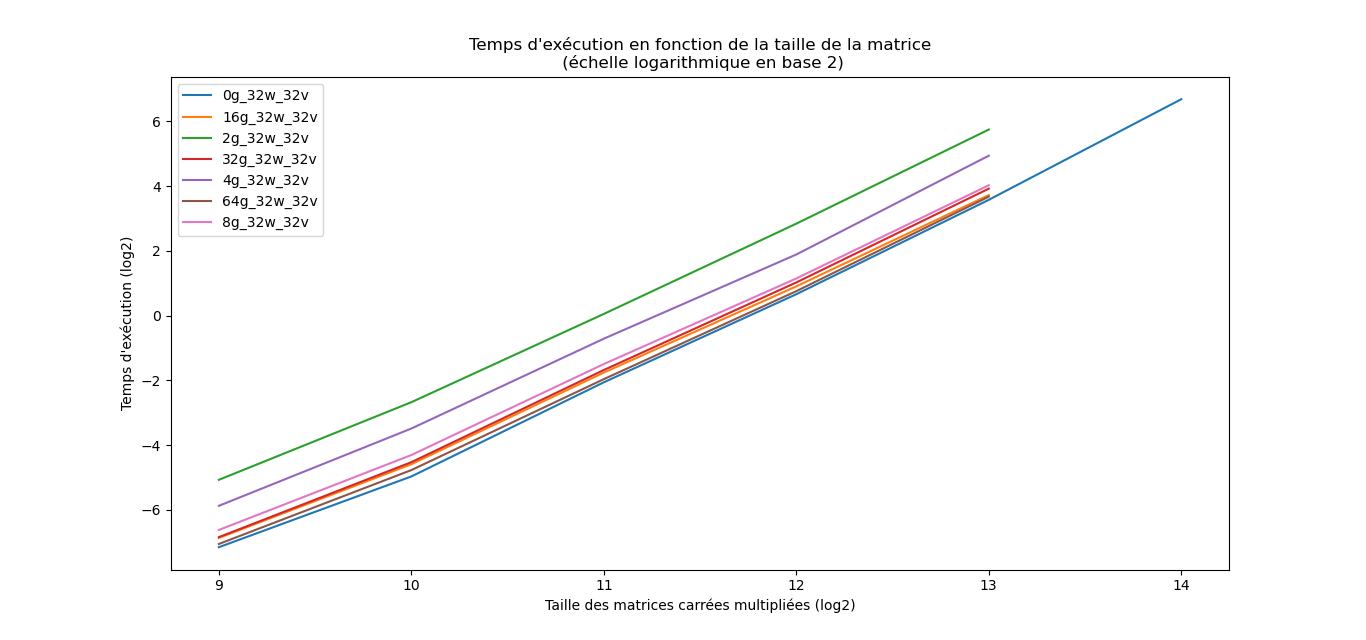
\includegraphics[width=\textwidth]{Gang_Log2.png}
	\caption{Evolution des temps de calcul en fonction du nombre de gangs}
\end{figure}

On constate ici que l'augmentation des gangs produit des résultats significatifs entre 2 et 128 gangs, et qu'au-delà il est plus difficile de quantifier les augmentations de performances, les courbes étant quasiment confondues (elles ont été retirées par souci de lisibilité). On note cependant que les temps de référence, c'est-à-dire les temps mesurés sans précision de nombre de gangs à la compilation, sont du même ordre que ceux mesurés pour le maximum de gangs spécifiés à la compilation.

\subsubsection{Mesures de performances}

On calcule de plus le nombre de \gls{flops} théoriques avec la formule suivante:

$$\mbox{flops} = \frac{(\mbox{taille des matrices})^2 \times (2 \times \mbox{taille des matrices} + 3)}{\mbox{temps d'exécution}}$$


\begin{figure}[!htb]

	\begin{subfigure}{\textwidth}
		\centering
		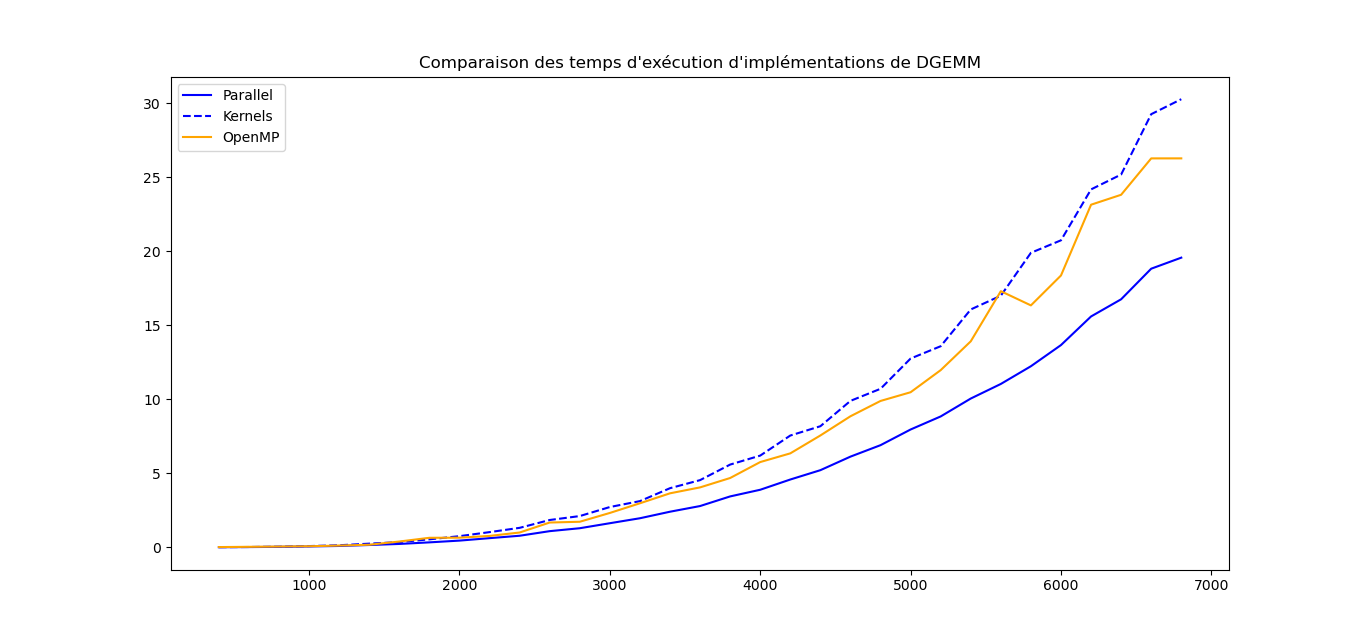
\includegraphics[width=\linewidth]{Time_DGEMM.png}
		\caption{Comparaison des temps d'exécution en fonction de la taille des matrices carrées}
		\label{fig:time_dgemm}
	\end{subfigure}

	\begin{subfigure}{\textwidth}
		\centering
		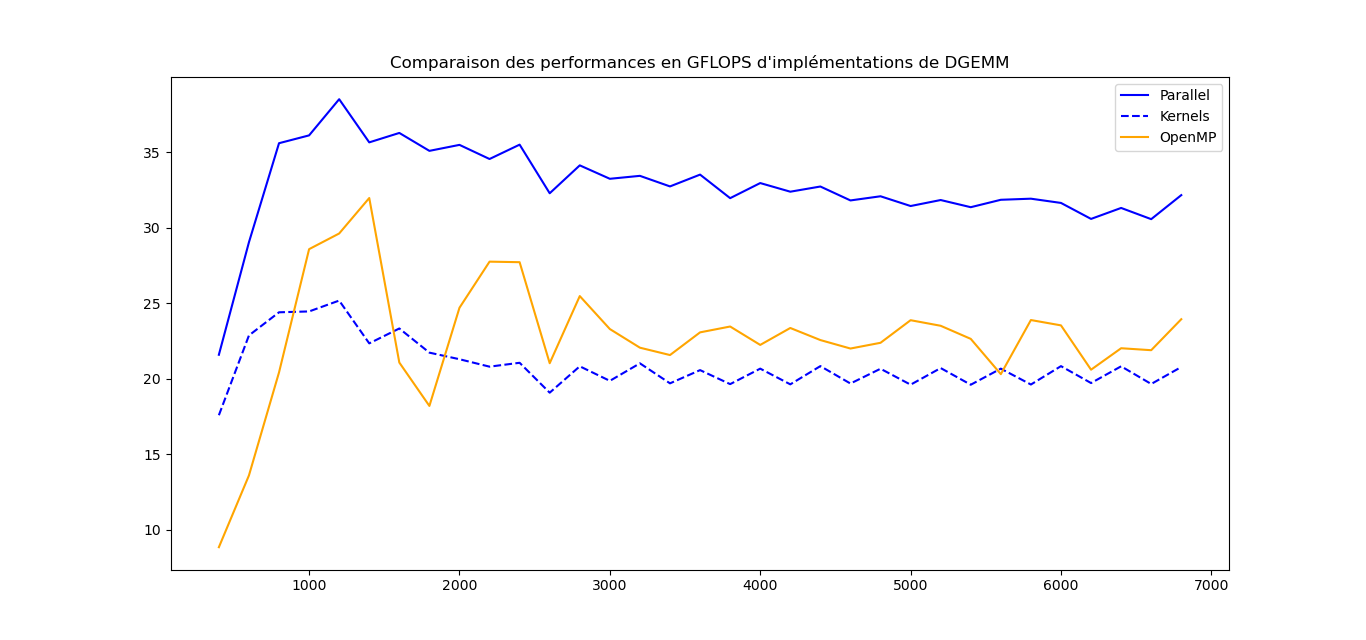
\includegraphics[width=\linewidth]{Flops_DGEMM.png}
		\caption{Comparaison des G\gls{flops} en fonction de la taille des matrices carrées}
		\label{fig:flops_dgemm}
	\end{subfigure}
	\caption{Etude de la multiplication généralisée de matrices carrées}
	\label{fig:dgemm_acc_ker_omp}
\end{figure}

On compare alors en figure \ref{fig:dgemm_acc_ker_omp} les résultats obtenus pour le codes compilé avec la directive \texttt{parallel} et les paramètres étudiés ci-dessus, pour le code compilé avec seulement la directive \texttt{kernels}, et pour le code compilé avec des directives \textit{OpenMP}. On observe sur la figure \ref{fig:flops_dgemm} que la directive \texttt{kernels} de \textit{OpenACC} suffit à obtenir des résultats comparables à ceux de \textit{OpenMP}, bien qu'un peu moins bons. En revanche, la directive \texttt{parallel} et une étude approfondie du nombre de gangs, de workers, et de la taille des vecteurs permettent une augmentation de performances de près de $40\%$.

\begin{figure}[!htb]

	\begin{subfigure}{\textwidth}
		\centering
		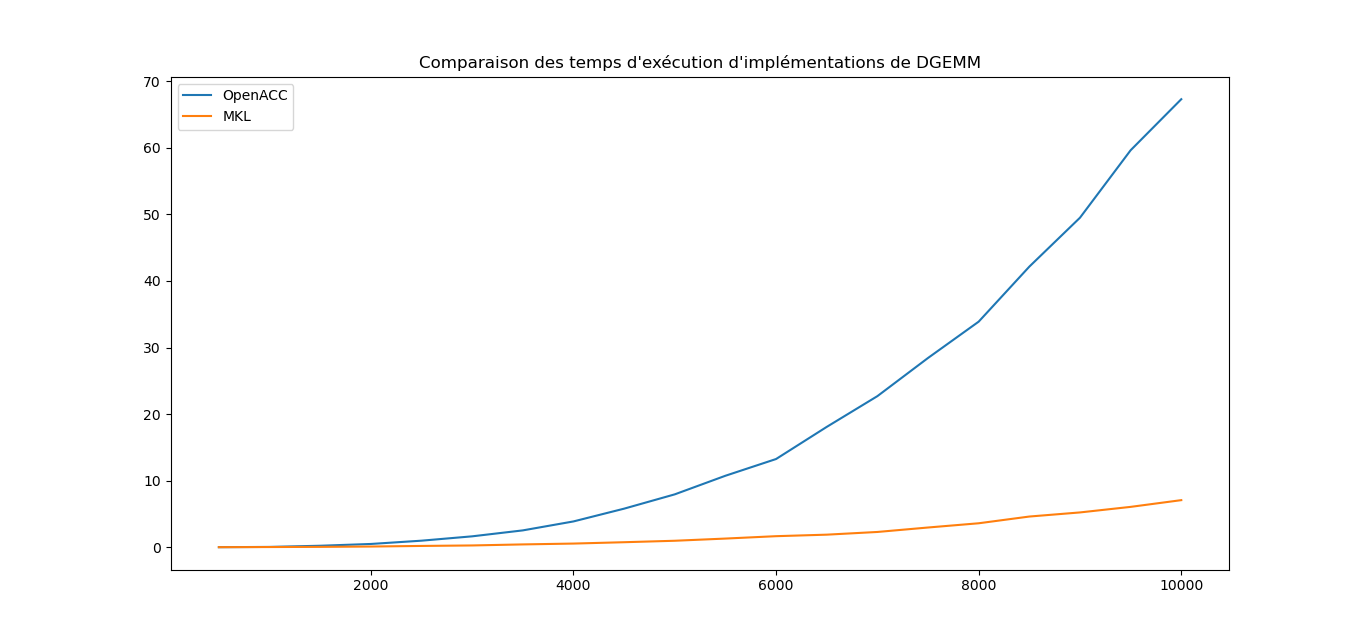
\includegraphics[width=\linewidth]{Time_OACC_MKL.png}
		\caption{Comparaison des temps d'exécution en fonction de la taille des matrices carrées}
	\end{subfigure}

	\begin{subfigure}{\textwidth}
		\centering
		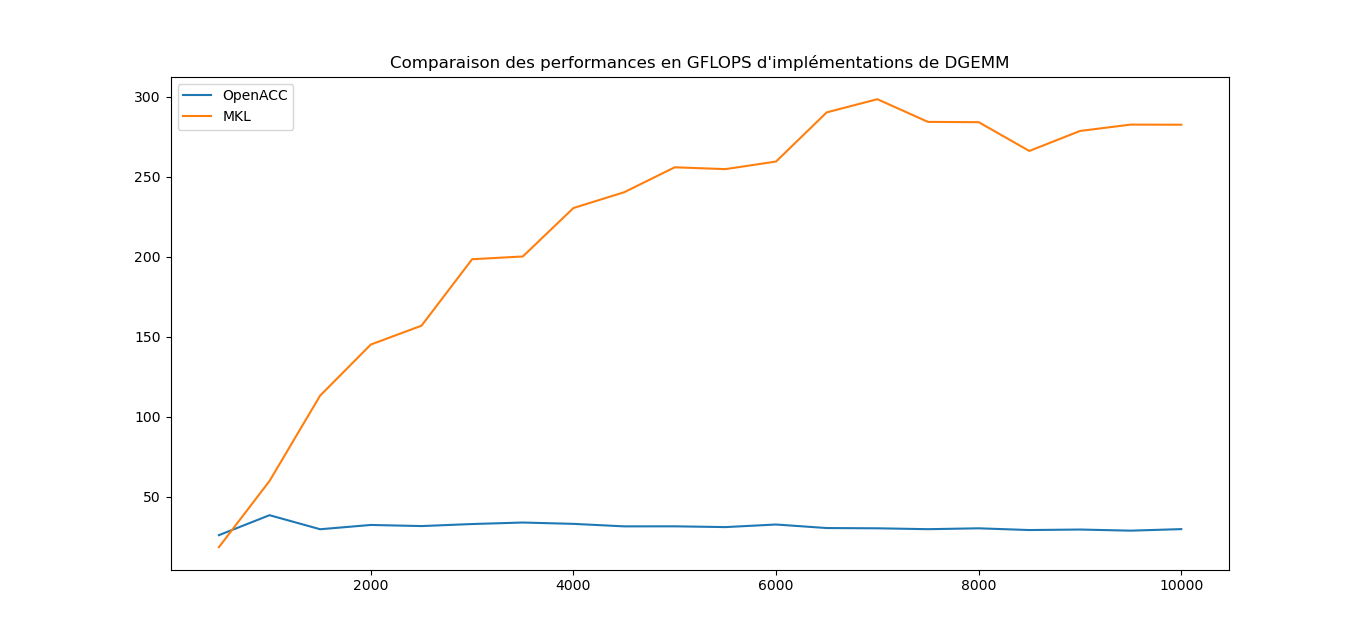
\includegraphics[width=\linewidth]{Flops_OACC_MKL.png}
		\caption{Comparaison des G\gls{flops} en fonction de la taille des matrices carrées}
	\end{subfigure}
	\caption{Etude de la multiplication généralisée de matrices carrées avec une implémentation optimisée (\textit{MKL})}
	\label{fig:dgemm_acc_mkl}
\end{figure}

On peut aussi comparer en figure \ref{fig:dgemm_acc_mkl} l'implémentation \textit{OpenACC} avec la directive \texttt{parallel} à un \textit{DGEMM} classique comme celui développé par \textit{Intel}, contenu dans la librairie \textit{MKL}. On constate ce qui était attendu: les performances de \textit{MKL} sont bien supérieures à celles obtenues par \textit{OpenACC}. On remarque même que malgré l'augmentation de la taille des matrices, les performances de ce dernier n'augmentent pas, contrairement à ce que l'on aurait pu penser.

\FloatBarrier

\subsection{Intégration par la méthode des trapèzes}

\subsubsection{Présentation}

L'intégration d'une fonction par la méthode des trapèzes consiste à découper l'aire sous la courbe étudiée en trapèzes successifs dont on sait aisément calculer puis sommer l'aire pour approximer l'intégrale recherchée.

\subsubsection{Code}

\begin{lstlisting}[caption={Implémentation de l'intégration par la méthode des trapèzes \textit{OpenACC}}]
double approx = 0.5 * (f(a) + f(b));
double h = (b - a) / N;
#pragma acc parallel loop reduction(+:approx)
for(int i = 0; i < N; i++){
	approx += f(a + i * h);
}
approx *= h;

#pragma acc routine
double f(double x){
	return 1/x;
}
\end{lstlisting}

\subsubsection{Détail des clauses}

\begin{itemize}
	\item \texttt{\#pragma acc parallel loop} On indique que la boucle qui suit est parallélisable.
	\item \texttt{\#reduction(+:approx)} On effectue ici une réduction sur la variable \texttt{approx} qui est la somme des aires de tous les trapèzes calculés.
	\item \texttt{\#pragma acc routine} On déclare ici que la fonction qui suit va être appelée et peut être parallélisée, voire vectorisée lors de ces appels.
\end{itemize}

~\\

\subsubsection{Mesure des performances}

Pour le calcul de l'aire de chaque trapèze, on considèrera que l'appel à une fonction extérieure ne correspond qu'à une opération à virgule flottante, soit $4$ opérations par itération en comptant la multiplication par $h$ et le calcul de $a + i * h$. On a donc la formule suivante:

$$\mbox{flops} = 4 \times \frac{\mbox{nombre de trapèzes}}{\mbox{temps d'exécution}}$$

\begin{figure}[!htb]

	\begin{subfigure}{\textwidth}
		\centering
		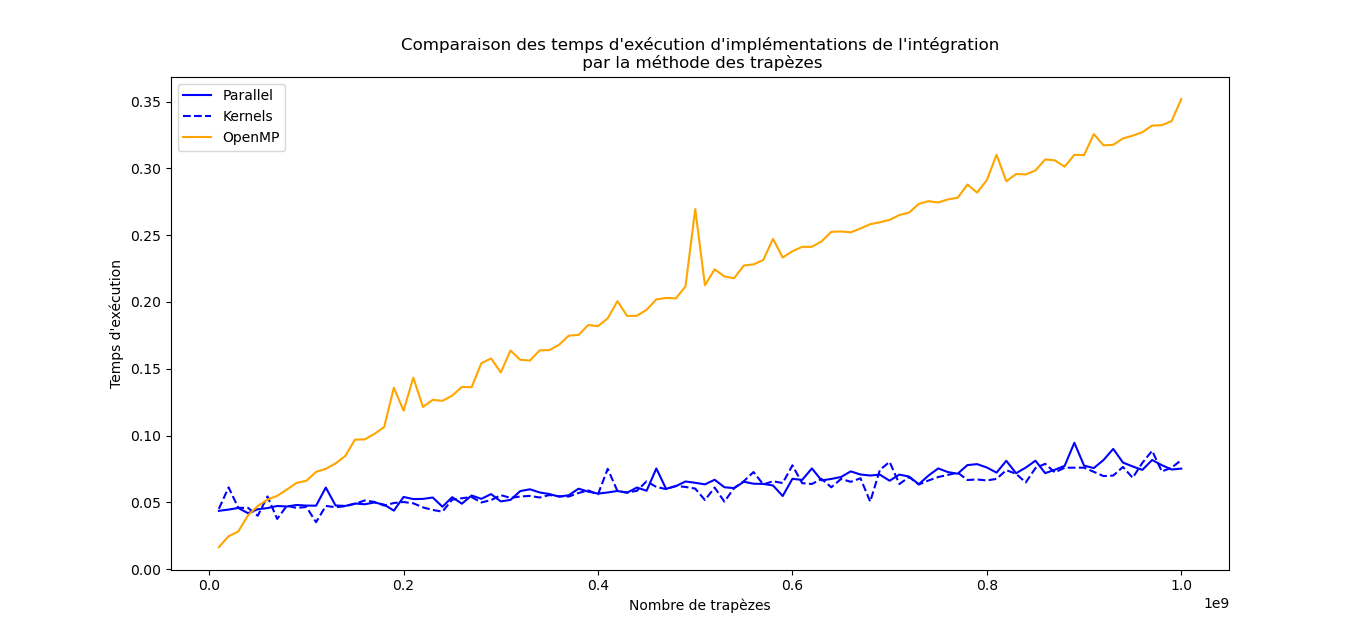
\includegraphics[width=\linewidth]{Time_itg.png}  
		\caption{Comparaison des temps d'exécution en fonction du nombre de trapèzes}
		\label{fig:time_itg}
	\end{subfigure}

	\begin{subfigure}{\textwidth}
		\centering
		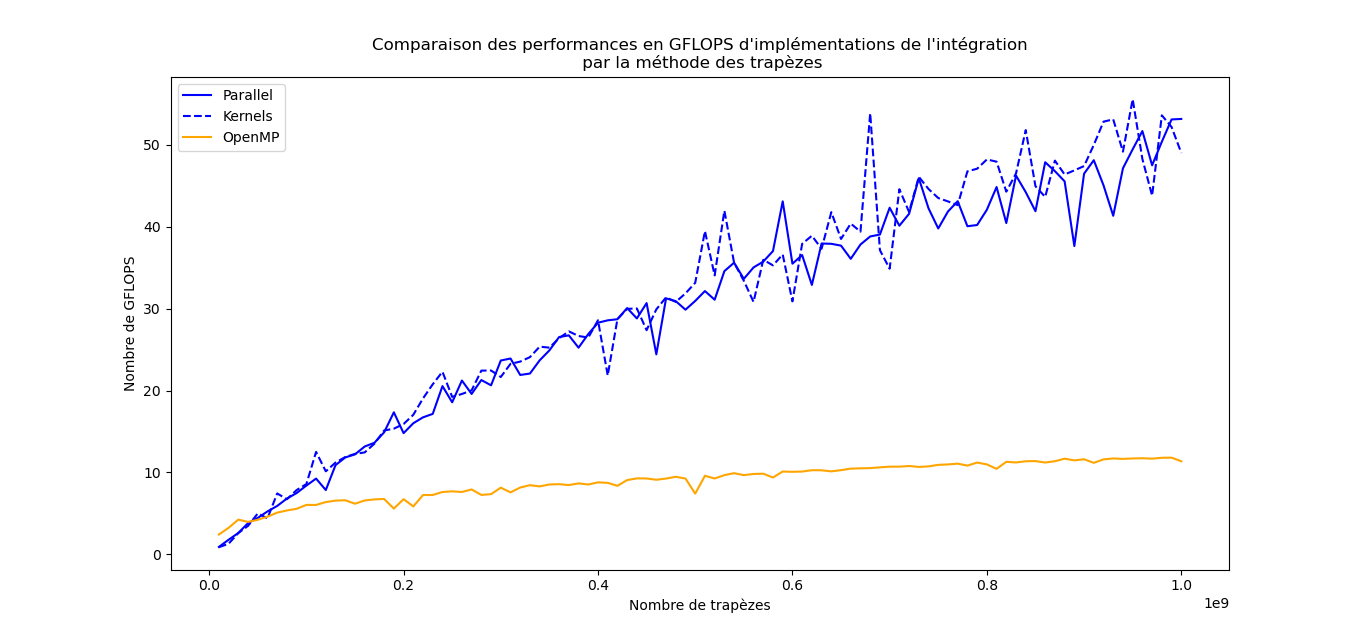
\includegraphics[width=\linewidth]{Flops_itg.png}  
		\caption{Comparaison des G\gls{flops} en fonction du nombre de trapèzes}
		\label{fig:flops_itg}
	\end{subfigure}
	\caption{Etude du calcul de $\int_{1}^{10^6}\frac{1}{x}dx$ par la méthode des trapèzes}
	\label{fig:itg_acc_ker_omp}
\end{figure}

On compare en figure \ref{fig:itg_acc_ker_omp} le calcul d'intégrales par la méthode des trapèzes implémenté avec \textit{OpenACC} en utilisant les directives \texttt{parallel} et \texttt{kernels}, et avec \textit{OpenMP}. On constate sur la figure \ref{fig:time_itg} que là où le temps d'exécution de l'implémentation \textit{OpenMP} augmente linéairement, le temps d'exécution de l'implémentation \textit{OpenACC} est quasiment constant, que l'on utilise la directive \texttt{parallel} ou \texttt{kernels}, ce qui correspond à l'augmentation linéaire du nombre de \textit{G\gls{flops}} en figure \ref{fig:flops_itg}, qui finit par dépasser celui de l'implémentation \textit{OpenMP}. Le \textit{\gls{gpu}} n'étant, comme le montre la figure \ref{fig:time_itg}, pas poussé à son maximum, le nombre maximum de \textit{G\gls{flops}} n'est pas représentatif de ses capacités. Les temps d'exécution sont trop courts pour faire une différence entre les deux implémentations \textit{OpenACC}, mais les calculs sont ici limités par les contraintes liées à la taille des variables. En effet, un \texttt{int} ne peut stocker des entiers au-dessus de $4 \times 10^{9}$, soit l'ordre auquel on s'est arrêté dans les mesures de performances, or les temps d'exécution restent en-dessous de la demie-seconde. C'est cependant suffisant pour déterminer que le \textit{\gls{gpu}} permet ici aussi de meilleures performances lorsque le nombre de trapèzes devient conséquent.

Pour obtenir une comparaison des temps d'exécution plus intéressante, il pourrait par exemple être judicieux d'étudier une fonctions plus complexe, comme un développement limité de fonction trigonométriques.

Il est important de noter que l'augmentation du nombre de trapèzes ici ne signifie pas nécessairement une augmentation de la précision du résultat, on constate en effet plutôt un cumul d'erreurs d'arrondis qui diminuent cette précision. Cependant on s'intéresse ici aux temps de calculs plus qu'au résultat.

\FloatBarrier

\subsection{Différences finies}

\subsubsection{Présentation}

Le calcul de différences finies est une méthode de recherche de solutions approchées à des équations aux dérivées partielles, qui consiste en une discrétisation du problème par un schéma numérique sur une grille structurée. On s'intéresse ici à l'exemple classique de l'équation de la chaleur.

\subsubsection{Code}

\begin{lstlisting}[caption={Implémentation des différences finies}]
double dt = 1./(double)(T-1);
double dx = 1./(double)(N-1);
#pragma acc data pcopy(C[0:N*N]) pcreate(Cnew[0:N*N])
{
for(int n = 0; n < T; n++){
#pragma acc parallel loop gang num_gangs(4096) vector_length(512)
	for(int i = 1; i < (N-1); i++){
#pragma acc loop vector
		for(int j = 1; j < (N-1); j++){
			Cnew[N * i + j] = (1 - 4 * dt / (dx * dx)) * C[N * i + j] + dt / (dx * dx) * (C[N * (i + 1) + j] + C[N * (i - 1) + j] + C[N * i + (j + 1)] + C[N * i + (j - 1)]);
		}
	}
	double* temp = Cnew;
	Cnew = C;
	C = temp;
}}
\end{lstlisting}

\subsubsection{Détail des clauses}

\begin{itemize}
	\item \texttt{\#pragma acc data} On déclare ici les déplacements de données que l'on souhaite effectuer, et l'on encadre par des accolades la zone concernée.
	\item \texttt{pcopyin(C[:]) pcopyout(Cnew[:])} On signale au compilateur que l'on souhaite copier en entrée le tableau \texttt{C}, et que l'on ne souhaite pas le récupérer à la fin. En revanche, on déclare vouloir récupérer les données calculées pour \texttt{Cnew}, mais sans prendre en compte les données qu'il contient déjà.
	\item Les directives \texttt{parallel}, \texttt{loop}, \texttt{gang}, \texttt{worker} et \texttt{vector}, ont les mêmes rôles de balisage et structuration de la \gls{paral}du code que précédemment  pour \textit{DGEMM}.
\end{itemize}

~\\

\subsubsection{Mesure des performances}

Pour chaque case, on effectue 12 opérations sur des flottants, on calcule donc les \gls{flops} théoriques par la formule suivante: 

$$\mbox{flops} = 12 \times \frac{\mbox{itérations} \times (\mbox{taille de la grille})^2}{\mbox{temps d'exécution}}$$


\begin{figure}[!htb]

	\begin{subfigure}{\textwidth}
		\centering
		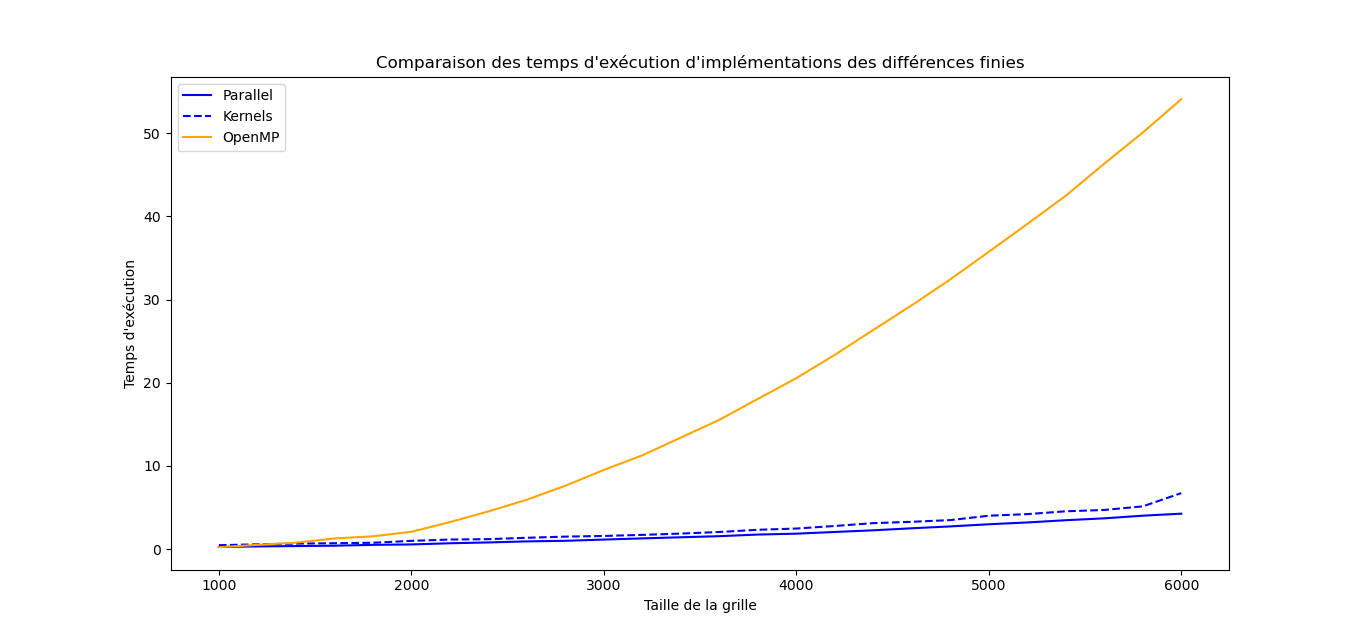
\includegraphics[width=\linewidth]{Time_diff.png}  
		\caption{Comparaison des temps d'exécution en fonction de la taille de la grille}
		\label{fig:time_diff}
	\end{subfigure}

	\begin{subfigure}{\textwidth}
		\centering
		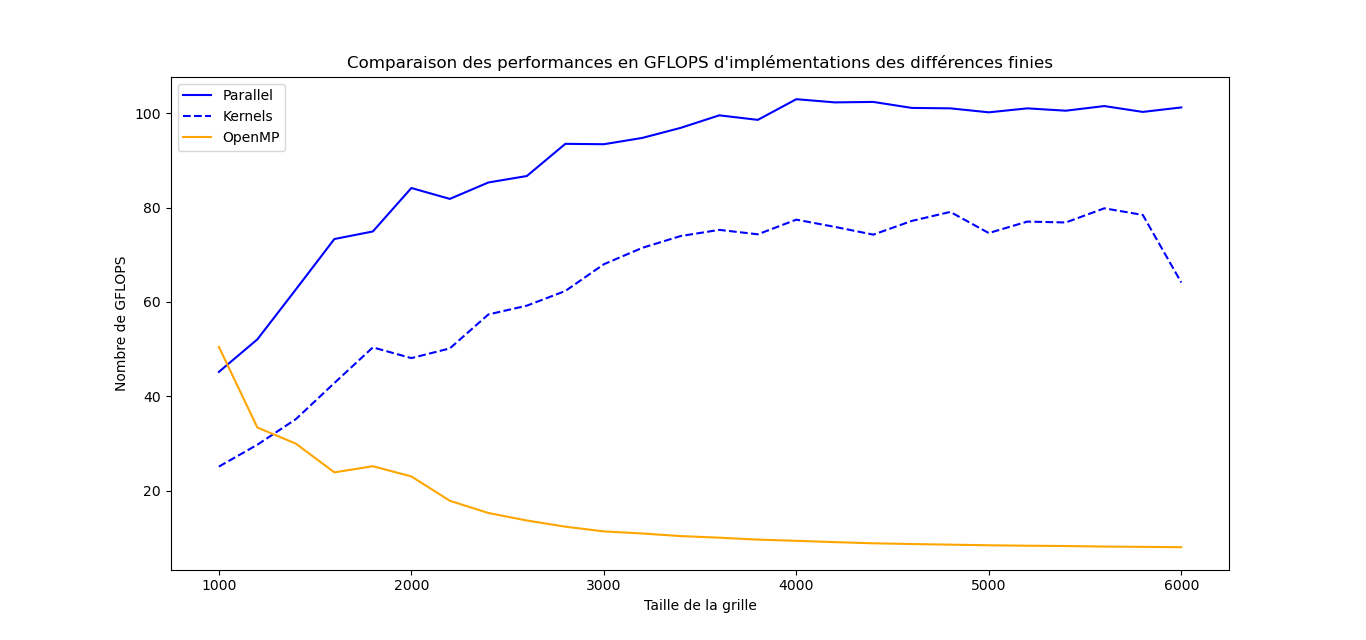
\includegraphics[width=\linewidth]{Flops_diff.png}  
		\caption{Comparaison des G\gls{flops} en fonction de la taille de la grille}
		\label{fig:flops_diff}
	\end{subfigure}
	\caption{Etude du calcul de différences finies pour les équations de la chaleur en deux dimensions pour 1000 itérations temporelles}
	\label{fig:diff_acc_ker_omp}
\end{figure}

On compare en figure \ref{fig:diff_acc_ker_omp} le calcul des différences finies implémenté avec \textit{OpenACC} en utilisant les directives \texttt{parallel} et \texttt{kernels}, et avec \textit{OpenMP}. On choisit ici de se limiter à $1000$ itérations temporelles, cependant il est à noter que les itérations temporelles ne pouvant être parallélisées, chacune demande la création d'un nouveau \textit{kernel}, ce qui est coûteux en temps. Sur de petites grilles et un grand nombre d'itérations, l'implémentation \textit{OpenMP} donnera donc de meilleurs résultats, comme le montre la figure \ref{fig:flops_diff}. En revanche, pour peu d'itérations mais une grande grille, l'implémentation \textit{OpenACC} sera plus efficace. On remarque de plus que la directive \texttt{kernels} donne des résultats intéressants par rapport à \textit{OpenMP}, mais qu'il est possible d'obtenir des performances autour de $25\%$ meilleures avec la directive \texttt{parallel} et une étude rapide des performances en fonction du nombre de gangs et de la taille des vecteurs. On remarque de plus que l'on arrive à atteindre les $100$ \textit{G\gls{flops}}, soit $5\%$ de la puissance nominale de la \textit{Tesla K80} en double précision, et ce avec très peu de directives.

\FloatBarrier

\section{Le cas des éléments finis}

\subsection{Exposé du problème}

On choisit ici d'utiliser \textit{OpenACC} sur un code plus conséquent, en l'occurence sur une implémentation de la méthode des éléments finis avec solveur de Jacobi. On se penchera plus particulièrement sur ce dernier.

Un solveur de Jacobi calcule itérativement la solution d'une équation de la forme $A . x = b$, en construisant la suite définie par la relation suivante: $u_{k+1} = (b - N . u_k) . D^{-1}$, avec $D$ diagonale, $N$ de diagonale nulle telle que $A = D + N$.

La matrice $N$ étant essentiellement constituée de zéros (\textit{matrice creuse}), la question du stockage de données s'est posée. En effet, un tableau complet plein de zéros est une grosse perte en termes de mémoire. On a donc commencé à la stocker sous la forme de trois listes, une contenant les valeurs non nulles, les deux autres contenant les colonnes et les lignes correspondant aux valeurs (format \textit{Coordinate list}). Cependant, ce format se prête mal à la \gls{paral} car le parcours simultané des valeurs peut entraîner du \textit{data race}. On a alors choisi de changer de format, en y préférant le format de \textit{Yale}, où le tableau de valeurs est ordonné par l'indice de la ligne des valeurs, la première liste contenant à l'indice $n$ l'emplacement, dans la liste des valeurs, où commencent les valeurs de la $n^e$ ligne, et la deuxième liste contenant la colonne correspondant à chaque valeur. Ce format permet un parcours de la matrice par lignes sans risquer de \textit{data race}.

\subsection{Abord du code}

La première chose que l'on remarque est que les itérations successives du solveur ne pourront pas êtres exécutées en parallèle, et que l'on pourra alors faire appel à la directive \texttt{async} qui permettra de ne pas perdre de temps lors de la préparation des \textit{kernels}.

Dans une première tentative de mettre en place \textit{OpenACC}, après la création de la clause \texttt{data} autour de la boucle principale du solveur, on se rend compte que sur un code important, la gestion des données est d'autant plus délicate qu'il y a beaucoup de variables, et qu'au sein d'une clause \texttt{data}, il est important de se demander, pour chaque opération, quelle est la variable sur laquelle on est en train de travailler, c'est-à-dire la variable en mémoire de l'\textit{hôte}, ou la copie (implicite ou non) dans la mémoire de l'\textit{accélérateur}.

De plus, s'il est recommandé d'effectuer d'abord la \gls{paral}, puis de s'occuper des transferts de mémoire, il s'avère, d'expérience, qu'il peut aussi être une bonne pratique de faire l'inverse, surtout lorsque la zone à paralléliser contient de nombreux \textit{kernels}. En effet, la construction progressive de ceux-ci permet de vérifier empiriquement que l'on effectue bien les calculs voulus sur les bonnes données, et que l'on n'a fait aucune omission dans les allocations et copies mémoires. 

De plus, avec les spécifications 2.7 d'\textit{OpenACC}, les \textit{deep copy} ne sont pas encore implémentées, et les structures ne sont pas correctement copiées sur l'\textit{accélérateur}. On a donc renommé tous les pointeurs vers des tableaux dans des structures pour éviter les erreurs de segmentation.

\subsection{Codes}

\begin{lstlisting}[caption="Optimisation du solveur de Jacobi"]
#pragma acc data copyin(N2_val[:N_nnz], diagA_val[:numDof], b_val[:numDof], N2_idzR[:numDof + 1], N2_idC[:N_nnz]) copy(u_val[:numDof]) create(Nu_val[:numDof])
{
  while (it < maxit && residual > tol){
#pragma acc parallel loop async
    for(int i=0; i<numDof; ++i){
      Nu_val[i] = 0.;
    }
#pragma acc parallel loop independent async
		for(int i = 0; i < numDof; i++){
			for(int j = N2_idzR[i]; j < N2_idzR[i + 1]; j ++){
				Nu_val[i] += N2_val[j] * u_val[N2_idC[j]];
			}
		}
    if((it % 1000) == 0){
      residual = 0;
#pragma acc parallel loop copy(residual) reduction(+:residual) async
      for(int n=0; n<numDof; n++){
        double tmp = diagA_val[n] * u_val[n] - Nu_val[n] - b_val[n];
        residual += tmp*tmp;
      }
#pragma acc wait
      residual = sqrt(residual);
    }
#pragma acc parallel loop async
    for(int i=0; i<numDof; ++i){
      u_val[i] = (Nu_val[i] + b_val[i]) / diagA_val[i];
    }
    it++;
  }
#pragma acc wait
}
\end{lstlisting}

~\\


\subsection{Détail des clauses}

\begin{itemize}
	\item \texttt{pragma acc data} Afin de limiter les transferts mémoire, on ne fait que copier les valeurs dont on a besoin dans la mémoire sans récupérer les éventuelles modifications à la fin de la zone via \texttt{copyin}. La seule valeur que l'on copie et que l'on récupère est la valeur de \texttt{u\_val} avec \texttt{copy}. Enfin, la variable \texttt{Nu\_val} ne contenant que des calculs temporaires, on ne fait que lui allouer un espace mémoire, sans copie de données.
	\item \texttt{pragma acc parallel loop async} A chacune des boucles, on se contente de signaler la \gls{paral} au compilateur, ce qui fait un nouveau \textit{kernel} à chaque boucle. En effet, on est obligé d'effectuer ces \textit{kernels} les uns à la suite des autres et non en concurrence pour éviter le \textit{data race}. Cependant, le paramètre \texttt{async} permet de laisser le \textit{\gls{cpu}} continuer à travailler sans attendre la fin des \textit{kernels}, et donc notamment de préparer les \textit{kernels} suivants sans attendre et de gagner du temps.
	\item \texttt{pragma acc wait} Si le paramètre \texttt{async} permet à l'\textit{hôte} de continuer ses calculs et donc de préparer les \textit{kernels} suivants, il continue à compter les itérations sans attendre la fin des \textit{kernels} de l'\textit{accélérateur}. Pour éviter que l'on arrive au maximum d'itérations sans avoir laissé l'\textit{accélérateur} terminer ses calculs, on ajoute cette directive pour que toutes les 1000 itérations, on resynchronise l'\textit{hôte} et l'\textit{accélérateur} après le calcul de la condition d'arrêt, avant de continuer les itérations si besoin. On ajoute aussi cette directive à la fin de la zone pour récupérer les valeurs exactes des variables, et éviter ainsi le \textit{data race}.
\end{itemize}

On note que le code obtenu est de complexité linéaire par rapport au nombre de valeurs non nulles dans la matrice $N$ et par rapport à la taille des matrices.

\subsection{Mesure des performances}

\begin{figure}[!htb]
	\centering
	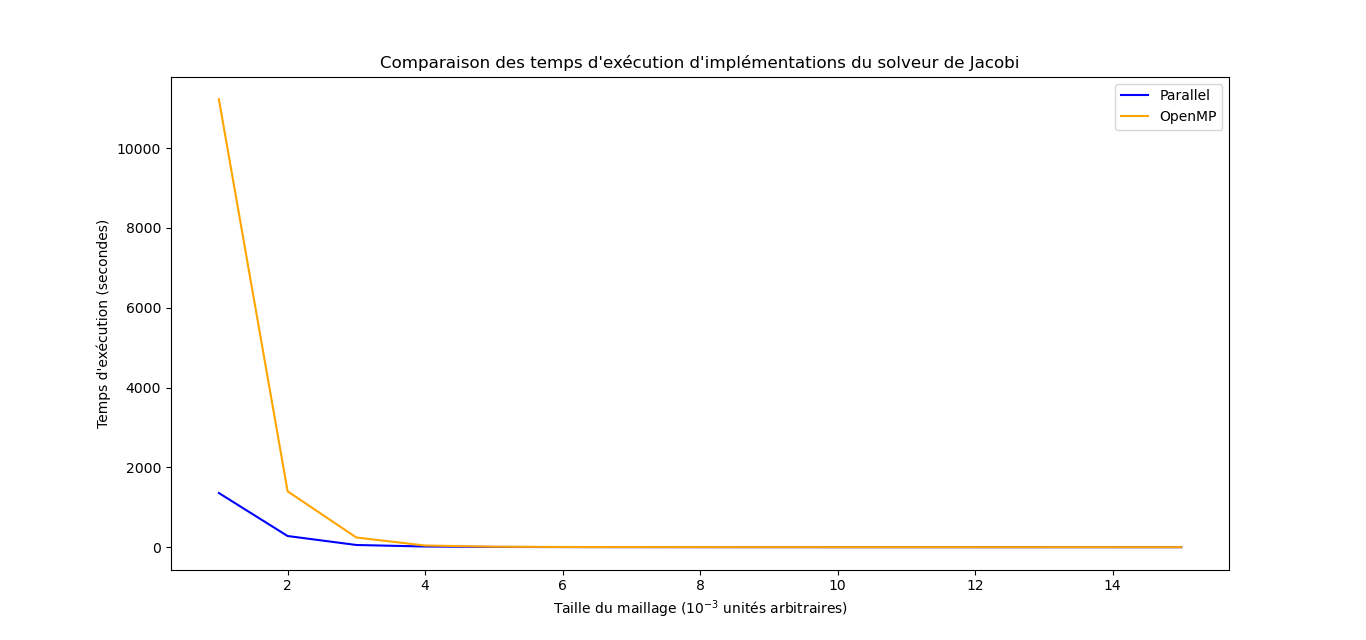
\includegraphics[width=\linewidth]{Time_elts.png}  
	\caption{Etude du temps d'exécution du solveur de Jacobi pour différentes tailles de maillage}
	\label{fig:elts_acc_omp}
\end{figure}

On obtient alors, après \gls{paral}, les résultats en figure \ref{fig:elts_acc_omp}. On constate que la \gls{paral} sur le \textit{\gls{gpu}} montre son efficacité lorsque le nombre d'éléments augmente, et ce d'autant plus que le code est de complexité linéaire. En effet, ce résultat est cohérent avec le fait que le cadençage du \textit{\gls{gpu}} soit plus faible que celui du \textit{\gls{cpu}}, mais avec un nombre d'unités de calcul indépendantes bien plus élevé. En effet, on voit que ces deux aspects se compensent sur un petit nombre d'éléments, mais que là où les itérations à effectuer sur chaque \gls{coeur} du \textit{\gls{cpu}} augmentent avec le nombre d'éléments à traiter, le \textit{\gls{gpu}} répartit d'autant plus le calcul et démontre d'autant plus son efficacité, étant jusqu'à 10 fois plus performant.

\section{Conclusion}

\subsection{Retour sur les résultats obtenus}

On a constaté durant cette étude que le standard \textit{OpenACC} permettait de porter facilement des codes sur \textit{\gls{gpu}}, via l'insertion de quelques directives de compilation dans le code.

Si l'on peut alors, sur des modifications comparables, obtenir des performances significativement meilleures que celles d'\textit{OpenMP} du fait de la puissance du \textit{\gls{gpu}}, on reste cependant loin derrière les performances théoriques annoncées par le constructeur du \textit{\gls{gpu}}. Il est donc raisonnable de penser que dans le cadre de tests de \gls{paral} sur \textit{\gls{gpu}}, \textit{OpenACC} puisse fournir une première approximation des possibilités, mais dans une perspective par exemple de simulation commerciale, une implémentation complète en \textit{\gls{cuda}} donnera probablement des résultats significativement meilleurs. On peut cependant envisager, du fait de la possibilité d'échanges de données entre des langages comme \textit{\gls{cuda}} ou \textit{OpenCL} avec \textit{OpenACC}, non abordée ici, que les portions critiques d'un code soient implémentées sur \textit{\gls{gpu}} dans un langage spécialisé, et que les portions annexes soient, elles, portées sur \textit{\gls{gpu}} via \textit{OpenACC} par souci de simplicité.

\subsection{Compétences acquises}

Ce stage m'a permis d'approfondir ma compréhension des \textit{\gls{gpu}s}, et même du fonctionnement d'un ordinateur dans son ensemble. J'ai pu m'initier au calcul distribué, ce qui est un atout majeur dans ma formation car applicable à un panel de domaines immense. Je pense, pour compléter ma formation, que je devrais m'initier à des langages spécialisés, comme \textit{\gls{cuda}} qui m'aurait été utile durant ce stage. Je souhaiterais aussi, à l'avenir, me pencher plus en détail sur le calcul scientifique à hautes performances, car c'est là aussi une compétence aussi intéressante que polyvalente.

L'expérience de travail à distance fut très intéressante mais à double tranchant. En effet, si j'ai été beaucoup plus libre sur mes horaires et plus généralement mon cadre de travail, il était parfois difficile de se motiver à travailler, surtout lorsque ma progression semblait dans une impasse. Heureusement, j'ai été bien entouré, tant par mes encadrants de stage qui ont su me guider efficacement malgré la distance, que par les camarades avec qui j'ai passé mon stage et qui m'ont aidé à maintenir une ambiance de travail sérieuse et productive.

L'expérience de recherche fut enrichissante, car c'est un domaine qui m'était jusqu'alors inconnu. La première difficulté fut de se trouver confronté à l'étendue infinie des possibles, de laquelle il m'a fallu tirer une structure à mon projet de recherche. Heureusement mes encadrants ont su me proposer un schéma à la fois suffisamment précis pour que mon stage ait un sens et un but, mais aussi suffisamment dense pour que je puisse faire moi-même mes choix sur ce que je souhaitais étudier en détail, et sur la méthodologie à employer. J'ai dû ensuite me résoudre à la frustration de la recherche peu couronnée de réussite, ou alors de réussites bien plus modestes qu'attendues, et du sentiment de lenteur dans la progression qui en résulte. Enfin, il a fallu se faire à l'idée que je n'aurais ni le temps, ni la volonté d'explorer à fond tout ce qu'il était possible d'explorer, ce qui ne fut pas facile à admettre. J'ai cependant apprécié la liberté que procure ce type de projet, la satisfaction d'une part d'avoir à exploiter les compétences acquises lors de mon cursus scolaire, et de me pousser intellectuellement, d'autre part de pouvoir choisir la méthodologie, les résultats à présenter et la façon de les obtenir.

\appendix

\newpage

Les annexes suivantes sont pour l'essentiel un résumé des directives, arguments et paramètres proposés par le standard \textit{OpenACC} 3.0 \cite{specs}.

\section{Directives de \gls{paral} \textit{OpenACC}}

\subsection{La directive \texttt{parallel}}

Cette directive sert à déclarer une zone du code comme parallèle, à la manière de \textit{OpenMP}. Cependant, dans la mesure où l'on cherche ici à utiliser la puissance de calcul du \textit{\gls{gpu}}, il faut ajouter en argument les données que l'on a besoin de copier vers la mémoire du \gls{gpu}, avec le paramètre \verb|copyin()|, et de récupérer depuis la mémoire du \textit{\gls{gpu}} en fin de calcul, avec le paramètre \verb|copyout()|, car ce transfert est coûteux et donc à limiter au maximum. On appelle cela l'\textit{offloading}.

\subsection{La directive \texttt{kernels}}

Cette directive sert à déclarer au compilateur qu'une zone est optimisable, tout en lui laissant la liberté de l'optimiser. On peut ensuite ajouter d'autres directives pour affiner cette \gls{paral} automatique, mais globalement, la directive \texttt{parallel} impose au compilateur une région parallèle, et l'efficacité de la \gls{paral} repose uniquement sur le programmeur. A l'inverse, \texttt{kernels} n'est qu'une incitation pour le compilateur à optimiser une zone, dans les limites de ses capacités d'analyse, et de ce qu'il identifiera comme sans risque pour l'intégrité du résultat. C'est donc une façon simple d'optimiser son code, et éventuellement de se faire une idée de ce qu'il est possible d'atteindre comme performances, mais il n'est pas garanti de tirer le maximum de performances atteignables à l'aide d'\textit{OpenACC}.

\subsection{La directive \texttt{seq}}

A l'inverse de \texttt{parallel} et \texttt{kernels}, cette directive sert à déclarer une portion de code comme séquentielle.

\subsection{La directive \texttt{loop}}

La directive \texttt{loop} donne une indication au compilateur sur le fait que la boucle qui suit est parallélisable. Elle peut s'employer seule, ou comme argument de \texttt{parallel} ou \texttt{kernels}. Elle n'est jamais superflue car elle donne une indication supplémentaire au compilateur sur la démarche à suivre.

La différence entre le multithreading sur \textit{\gls{cpu}} et sur \textit{\gls{gpu}} est que le \textit{\gls{gpu}} est constitué d'un nombre bien plus important d'unités de calcul indépendantes, organisées en groupes eux-mêmes indépendants. Il est donc possible d'exécuter en parallèle des portions de boucles sur différents groupes d'unités de calcul appelés \verb|gang| à l'aide de la directive éponyme, à la manière de la directive \verb|parallel for| de \textit{OpenMP}. Cependant, au sein même de cette \gls{paral}, il est possible d'effectuer une "sous \gls{paral}" sur les unités de calcul indépendantes, appelées \verb|worker| à l'aide de la directive éponyme, qui peuvent alors se partager une autre boucle, au sein de laquelle il est possible d'effectuer une vectorisation des calculs à l'aide de la directive \verb|vector|.

\subsection{La directive \texttt{routine}}

Elle permet de déclarer au code une fonction qui sera appelée dans une boucle à paralléliser. Il est important de déclarer ses fonctions de cette façon car elles risqueraient sinon d'empêcher des \gls{paral}s.

\subsection{La directive \texttt{atomic}}

Identique à son équivalent \textit{OpenMP}, cet argument permet de préciser le comportement des threads vis-à-vis d'une variable partagée lorsque l'argument \texttt{reduction} est trop restrictif. Il est évidemment moins efficace car plus permissif.

\section{Les arguments \textit{OpenACC}}

Aux directives s'ajoutent des arguments qui précisent le comportement à adopter pour le compilateur.

\subsection{L'argument \texttt{reduction}}

Identique à son équivalent \textit{OpenMP}, cet argument permet de préciser le comportement à avoir vis-à-vis d'une variable dont chaque thread a une copie locale. Il peut s'agir d'une somme, d'une addition, d'un calcul de minimum, de maximum, ou un certain nombre d'opérations bits à bits.

\subsection{L'argument \texttt{private}}

Cet argument permet de préciser les variables dont chaque thread doit avoir une copie locale. Il est à noter que les variables déclarées dans une boucle seront locales, les itérateurs seront locaux, les variables consultées seront locales et initialisées à leurs valeurs avant la boucle à chaque itération.

\subsection{Les arguments \texttt{gang}, \texttt{workers} et \texttt{vector}}

Lors de la \gls{paral} de calculs sur \textit{\gls{gpu}}, il existe plusieurs niveaux de parallélisme. En effet, une carte graphique est composée de nombreuses unités de calcul indépendantes, appelées \texttt{workers}, qui sont organisés en groupes appelés \texttt{gangs}, et qui, comme les \gls{coeur}s d'un \textit{\gls{cpu}}, peuvent effectuer des calculs vectorisés. Il y a donc trois niveaux de parallélisme à considérer, et il est intéressant, au sein de plusieurs boucles imbriquées, d'étudier les différentes répartitions des tâches pour en déterminer la plus efficace. En effet, après chaque directive \texttt{loop}, il est possible de préciser sur quel niveau on souhaite décomposer la boucle, avec les arguments \texttt{gang}, \texttt{worker} et \texttt{vector}. Ils sont a priori toujours dans cet ordre, et l'argument \texttt{vector} est a priori toujours sur la boucle la plus intérieure (en effet il n'est possible de vectoriser que des calculs sur des tableaux). 

\subsection{L'argument  \texttt{collapse()}}

Cet argument permet, lors d'une imbrication importante de boucles, de ne plus itérer que sur un seul indice pour faciliter la vectorisation. L'entier en paramètre précise combien de boucles on souhaite combiner.


\section{Gestion de la mémoire}

La gestion de la mémoire est l'un des points clefs du calcul sur \textit{\gls{gpu}}. En effet, le transit de données entre la mémoire du \textit{\gls{cpu}}, la mémoire vive, et la mémoire du \textit{\gls{gpu}} est très coûteux en temps, il est donc essentiel de savoir bien organiser ses données et ne pas faire de déplacements superflus. On appelle ces tranfserts de mémoire l'\textit{offloading}. Il est possible d'ajouter localement aux directives déjà présentes des arguments de déplacement de données spécifiques, mais le plus simple est de créer autour de la zone à paralléliser une clause \texttt{data}.

\subsection{La clause \texttt{data}}

Comme toutes les directives d'\textit{OpenACC}, elle se déclare de la façon suivante:

\texttt{\#pragma acc data}

On y ajoute ensuite des arguments de déplacement de données pour préciser ce que l'on veut faire. Comme précisé précédemment, ces arguments peuvent être ajoutés aux différentes directives, notamment \texttt{parallel}, \texttt{loop}, ou \texttt{kernels}, au risque cependant de créer des déplacements inutiles.

On précisera entre parenthèses les tableaux de données que l'on souhaite transférer, suivi entre crochets de l'indice de l'entrée à laquelle on veut commencer le transfert, suivi du nombre d'entrées à transférer. Par exemple, \texttt{A[0:N]} permettra de transférer les données de l'indice \texttt{0} à l'indice \texttt{N}. On notera qu'il est en théorie possible d'écrire \texttt{A[:]} pour transférer toutes les données contenues dans \texttt{A}, mais il est possible que l'\textit{hôte} n'arrive pas à trouver de lui-même le début et la fin du tableau.

\subsection{L'argument \texttt{copyin()}}

Cet argument sert à copier les données spécifiées dans la mémoire de l'\textit{accélérateur} pour y faire des opérations. Ces données ne seront pas actualisées dans la mémoire du \textit{\gls{cpu}} ni dans la RAM et les potentielles modifications effectuées dessus seront perdues à la fin de la portion de code concernée par la directive.

\subsection{L'argument \texttt{copyout()}}

Cet argument sert à créer une zone de données dans la mémoire de l'\textit{accélérateur} de la taille des éléments passés en paramètre, zone dans laquelle on pourra stocker les résultats des opérations effectuées dans la portion de code concernée par la directive, et qui ensuite sera exportée dans la RAM, remplaçant les données présentes s'il y en avait. 

\subsection{L'argument \texttt{copy()}}

Cet argument cumule les fonctions de \texttt{copyin()} et \texttt{copyout()}. Il est donc utile pour les données qui ont déjà été initialisées, sur lesquelles on souhaite faire des modifications qui seront conservées pour la suite de l'exécution.

\subsection{L'argument \texttt{present()}}

Cet argument sert à spécifier que les éléments passés en paramètre sont déjà présents dans la mémoire du \textit{\gls{gpu}} (suite à une directive antérieure) et que l'on cherche à les réutiliser (attention, il n'est pas certain que les modifications effectués hors \textit{\gls{gpu}} soient actualisées).

\subsection{L'argument \texttt{update()}}

Cet argument permet de demander à l'hôte de simplement résoudre les deltas entre un jeu de données déjà en mémoire de l'\textit{accélérateur} qui a été actualisé, par un autre \textit{accélérateur} ou par l'\textit{hôte}, au lieu de le copier totalement.

\subsection{Le préfixe \texttt{p-}}

Les arguments ci-dessus ont vocation à disparaître au profit des mêmes précédés de "\texttt{p}" (\textit{ex: } \texttt{pcopyin}, \texttt{pcreate}...), qui signifie "\textit{Present or ...}", et qui a pour effet que le \textit{\gls{cpu}} vérifie si les données ne sont pas déjà présentes avant de les copier, ce qui peut faire gagner un temps précieux si la région \texttt{data} est à l'intérieur d'une boucle par exemple.

\subsection{Les structures en C++}

On notera qu'il est possible d'utiliser des classes en C++ avec des accélérateurs, il suffit d'ajouter les directives \texttt{OpenACC} nécessaires aux différents constructeurs et destructeurs, mais cela ne sera pas détaillé ici.

\section{Affinage du code}

Une fois que le code a été parallélisé et que les transferts de mémoire ont été gérés, il est toujours possible de gagner en performances en ajustant le code à l'\textit{accélérateur} sur lequel on veut le faire tourner. Le code perd alors de sa portabilité, mais il devient possible d'obtenir de bien meilleures performances.

\subsection{Gestion des gangs, workers et vecteurs}

Par défaut, une fois la structure de la \gls{paral} indiquée au compilateur, celui-ci va déterminer les nombres de \texttt{gangs}, de \texttt{workers} et la taille des \texttt{vectors} automatiquement. Il est cependant possible de lui préciser ces valeurs dans la limite de ce que l'\textit{accélérateur} peut supporter. Dans le cas d'une région de type \texttt{kernels}, on précisera directement les nombres de \texttt{gangs}, \texttt{workers}, et la taille des \texttt{vecteurs} en paramètres des arguments correspondants. Dans le cas d'une région de type \texttt{parallel}, on précisera ces valeurs après la directive \texttt{parallel} avec les arguments \texttt{num\_gangs()}, \texttt{num\_workers()} et \texttt{vector\_length()}. Il est recommandé de faire différents essais afin de trouver les paramètres optimaux. Attention cependant, des valeurs trop élevées ne produiront pas nécessairement d'erreurs à la compilation, mais à l'exécution.

\subsection{Gestion des \textit{kernels} et de la synchronicité}

Lors de l'exécution d'un programme sur \textit{\gls{gpu}}, les ensembles de calculs successifs sont rassemblés en un noyau de calcul, que l'on appelle un \textit{kernel}. Pour chaque portion de code exécutée sur \textit{\gls{gpu}}, un \textit{kernel} doit être mis en place par l'\textit{hôte}. C'est-à-dire qu'il détermine la répartition des calculs sur l'\textit{accélérateur} pour chaque appel. Une fois que cette préparation est faite, les instructions sont envoyées à l'\textit{accélérateur} qui ne fait qu'exécuter les calculs. L'\textit{hôte} attend alors qu'un \textit{kernel} soit terminé avant d'en mettre en place un nouveau. Or, le temps d'attente de l'\textit{hôte} pourrait parfois être employé à effectuer des opérations indépendantes, comme par exemple la mise en place d'un nouveau \textit{kernel}. Il est alors possible de dire à l'hôte de ne pas attendre la fin d'un \textit{kernel} pour effectuer des opérations en ajoutant l'argument \texttt{async} aux directives de \gls{paral} de boucles. Ensuite, lorsqu'il est nécessaire d'attendre que tous les calculs sur l'\textit{accélérateur} aient été exécutés, on peut insérer la directive \texttt{wait}, qui attendra la fin de l'exécution des \textit{kernels} pour lancer les opérations suivantes.

Il est à noter que l'argument \texttt{async} ne compromet pas l'ordre d'exécution des opérations, il permet juste d'exécuter des opérations sur l'\textit{hôte} pendant que des opérations sont effectuées sur l'\textit{accélérateur}. Il faudra alors porter une attention toute particulière aux données traitées, car chacun des deux agira sur ses copies locales des variables, ce qui peut compromettre par exemple la terminaison d'une boucle si l'\textit{accélérateur} effectue des opérations sur la variable de terminaison alors que c'est l'\textit{hôte} qui est en charge de vérifier la terminaison, car sa variable ne sera jamais modifiée.

Il est aussi possible de créer plusieurs files d'exécution, et de préciser dans quelle file on souhaite voir un ensemble d'instruction exécuté en ajoutant en paramètre de l'argument \texttt{async()} le numéro de la file d'exécution. Les éléments d'une même file d'exécution sont exécutés séquentiellement, les éléments de files différentes sont exécutés concurrentiellement. Il devient alors possible d'effectuer des calculs sur une partie des données, et de transférer les résultats pendant que l'on lance d'autres calculs simultanément.  


\subsection{Gestion de plusieurs accélérateurs}

Il est possible qu'il y ait plusieurs accélérateurs disponibles au sein d'une même machine. Il est alors intéressant d'exploiter cette opportunité. On peut récupérer le nombre d'accélérateurs de type \texttt{device\_type} via la fonction \\ \texttt{acc\_get\_num\_device(device\_type)}, et le numéro de l'\textit{accélérateur} sur lequel on travaille via \texttt{acc\_get\_device\_num(device\_type)}. On peut changer l'accélérateur sur lequel on travaille via l'instruction \\ \texttt{acc\_set\_device\_num(n, device\_type)}. Le travail par bloc devient alors d'autant plus pertinent.

\newpage



\listoffigures

\newpage

\bibliography{Rapport}
\bibliographystyle{ieeetr}

\end{document}
